\documentclass[a4paper,10pt]{article}
\usepackage[english]{babel}

%Plaatjes
\usepackage{graphicx}
\usepackage{float}
\usepackage{subcaption}
\captionsetup{subrefformat=parens}
\usepackage[font=small,format=plain,labelfont=bf,textfont=it]{caption}

%Accenten
\usepackage{lmodern}
\usepackage[utf8]{inputenc} 
\usepackage[T1]{fontenc}

%Referenties
\usepackage{varioref}
\usepackage{hyperref}
\usepackage[noabbrev]{cleveref}

\title{Point Normal Gallery}
\author{Laura Baakman \and Rick van Veen}

\begin{document}
\makeatletter
\g@addto@macro\@maketitle{
\begin{figure}[H]
    \setlength{\linewidth}{\textwidth}
    \setlength{\hsize}{\textwidth}
    \centering
	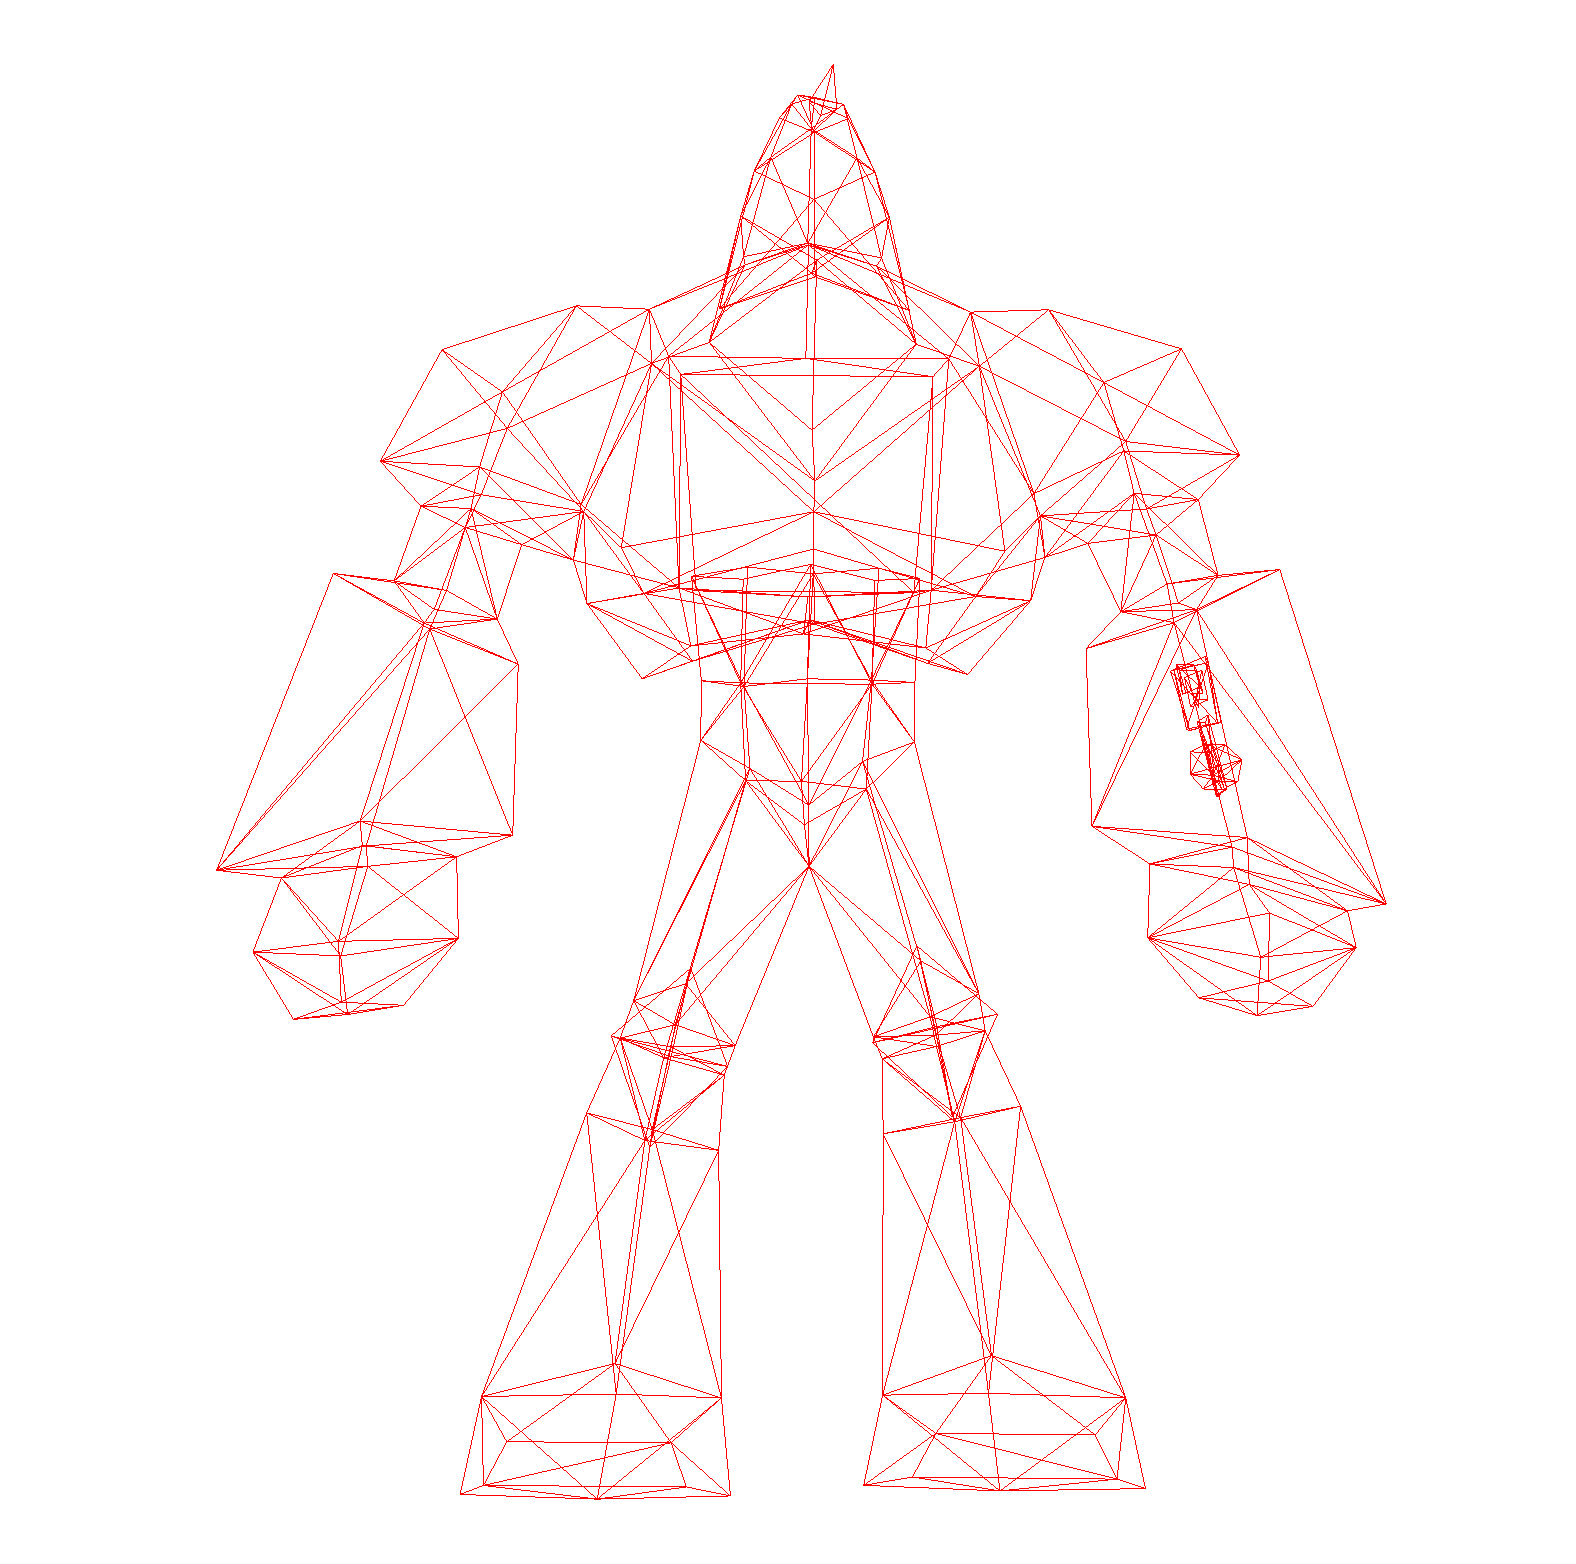
\includegraphics[width=\textwidth]{enforcer_wireframe.png}
	\caption{The input mesh.}		
	\label{fig:enforcerWireframe}	
    \end{figure}
}
\maketitle

\begin{figure}
	
\includegraphics[width=\textwidth]{enforcer_flat.png}
	\caption{The input mesh with flat shading and no lighting. Compare the contours of this model with the models where the outer tessellation levels is high, e.g. \cref{fig:phong:i5o5}, and with the model where the outer tessellation levels are low, but the inner levels are high, e.g. \cref{fig:phong:i9o1} to see how the point-normal triangles improve the contours.}
	\label{fig:enforcerFlat}	
\end{figure}

\begin{figure}
	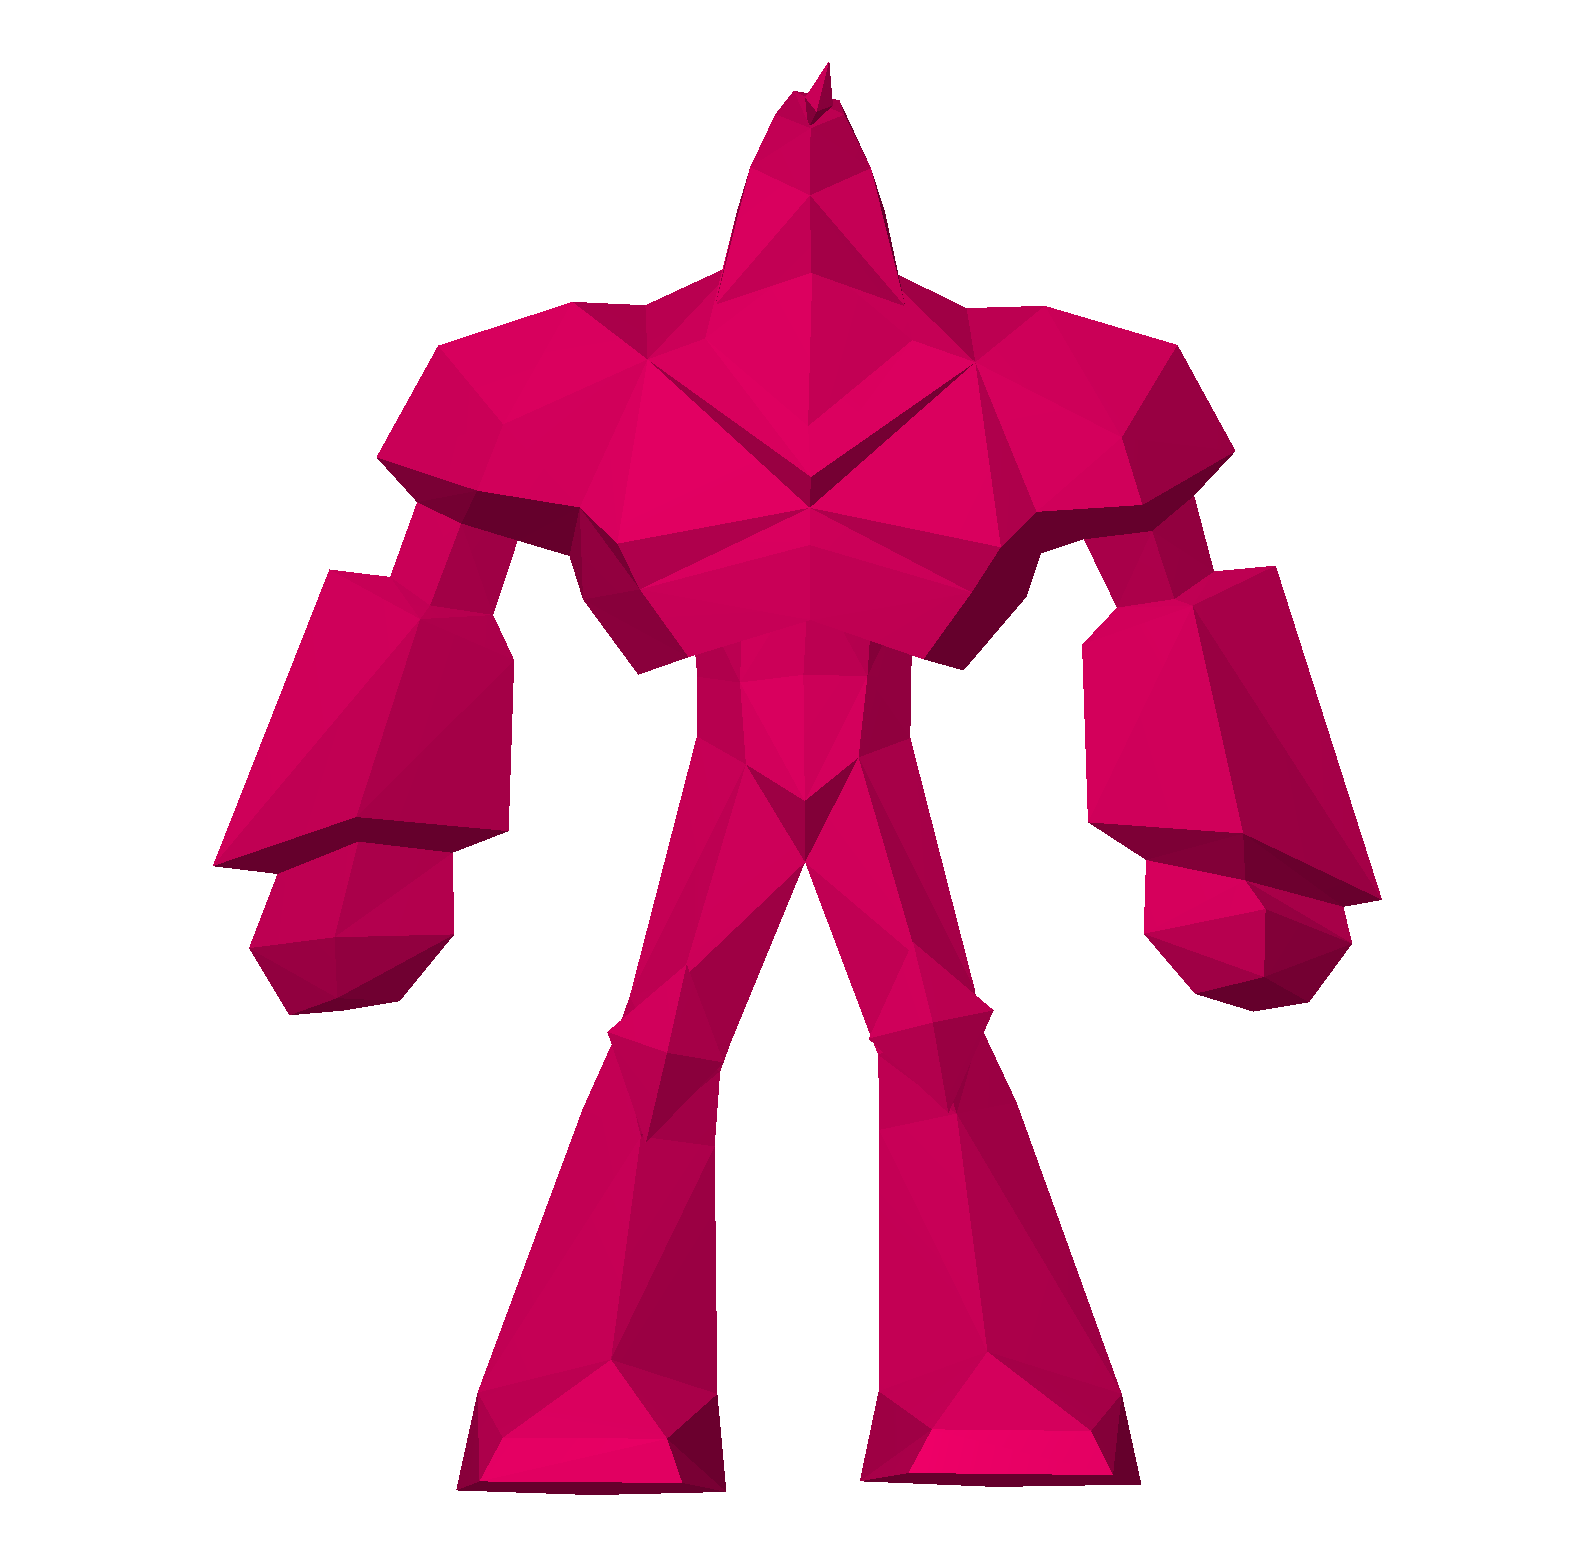
\includegraphics[width=\textwidth]{enforcer_flat_phong.png}
	\caption{The input mesh with flat shading and the Phong illumination model.}	
\end{figure}

\begin{figure}
	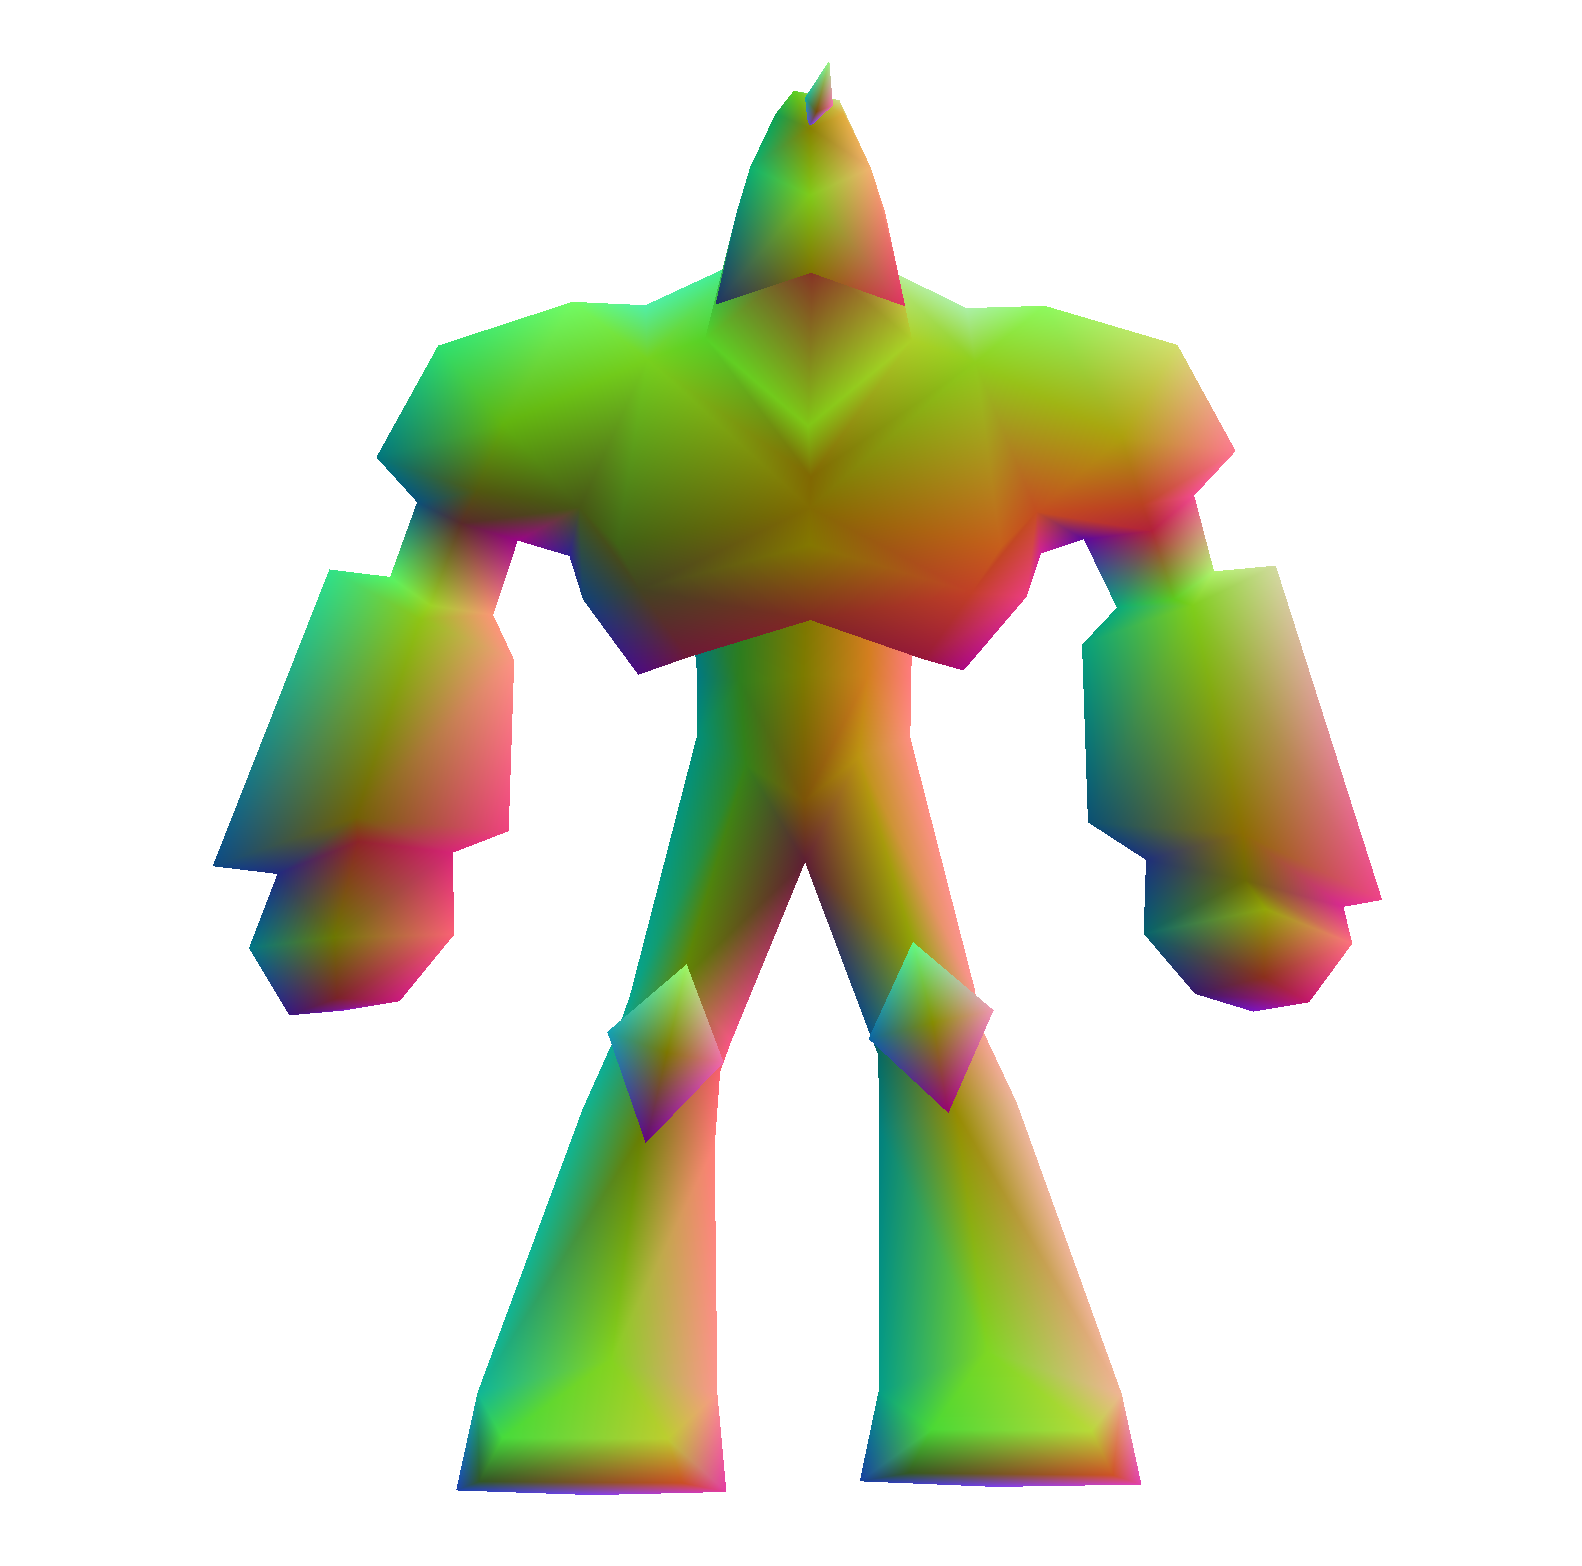
\includegraphics[width=\textwidth]{enforcer_normals.png}
	\caption{The input mesh colored based the scaled input normals.}		
	\label{fig:enforcerNormals}	
\end{figure}

\begin{figure}
	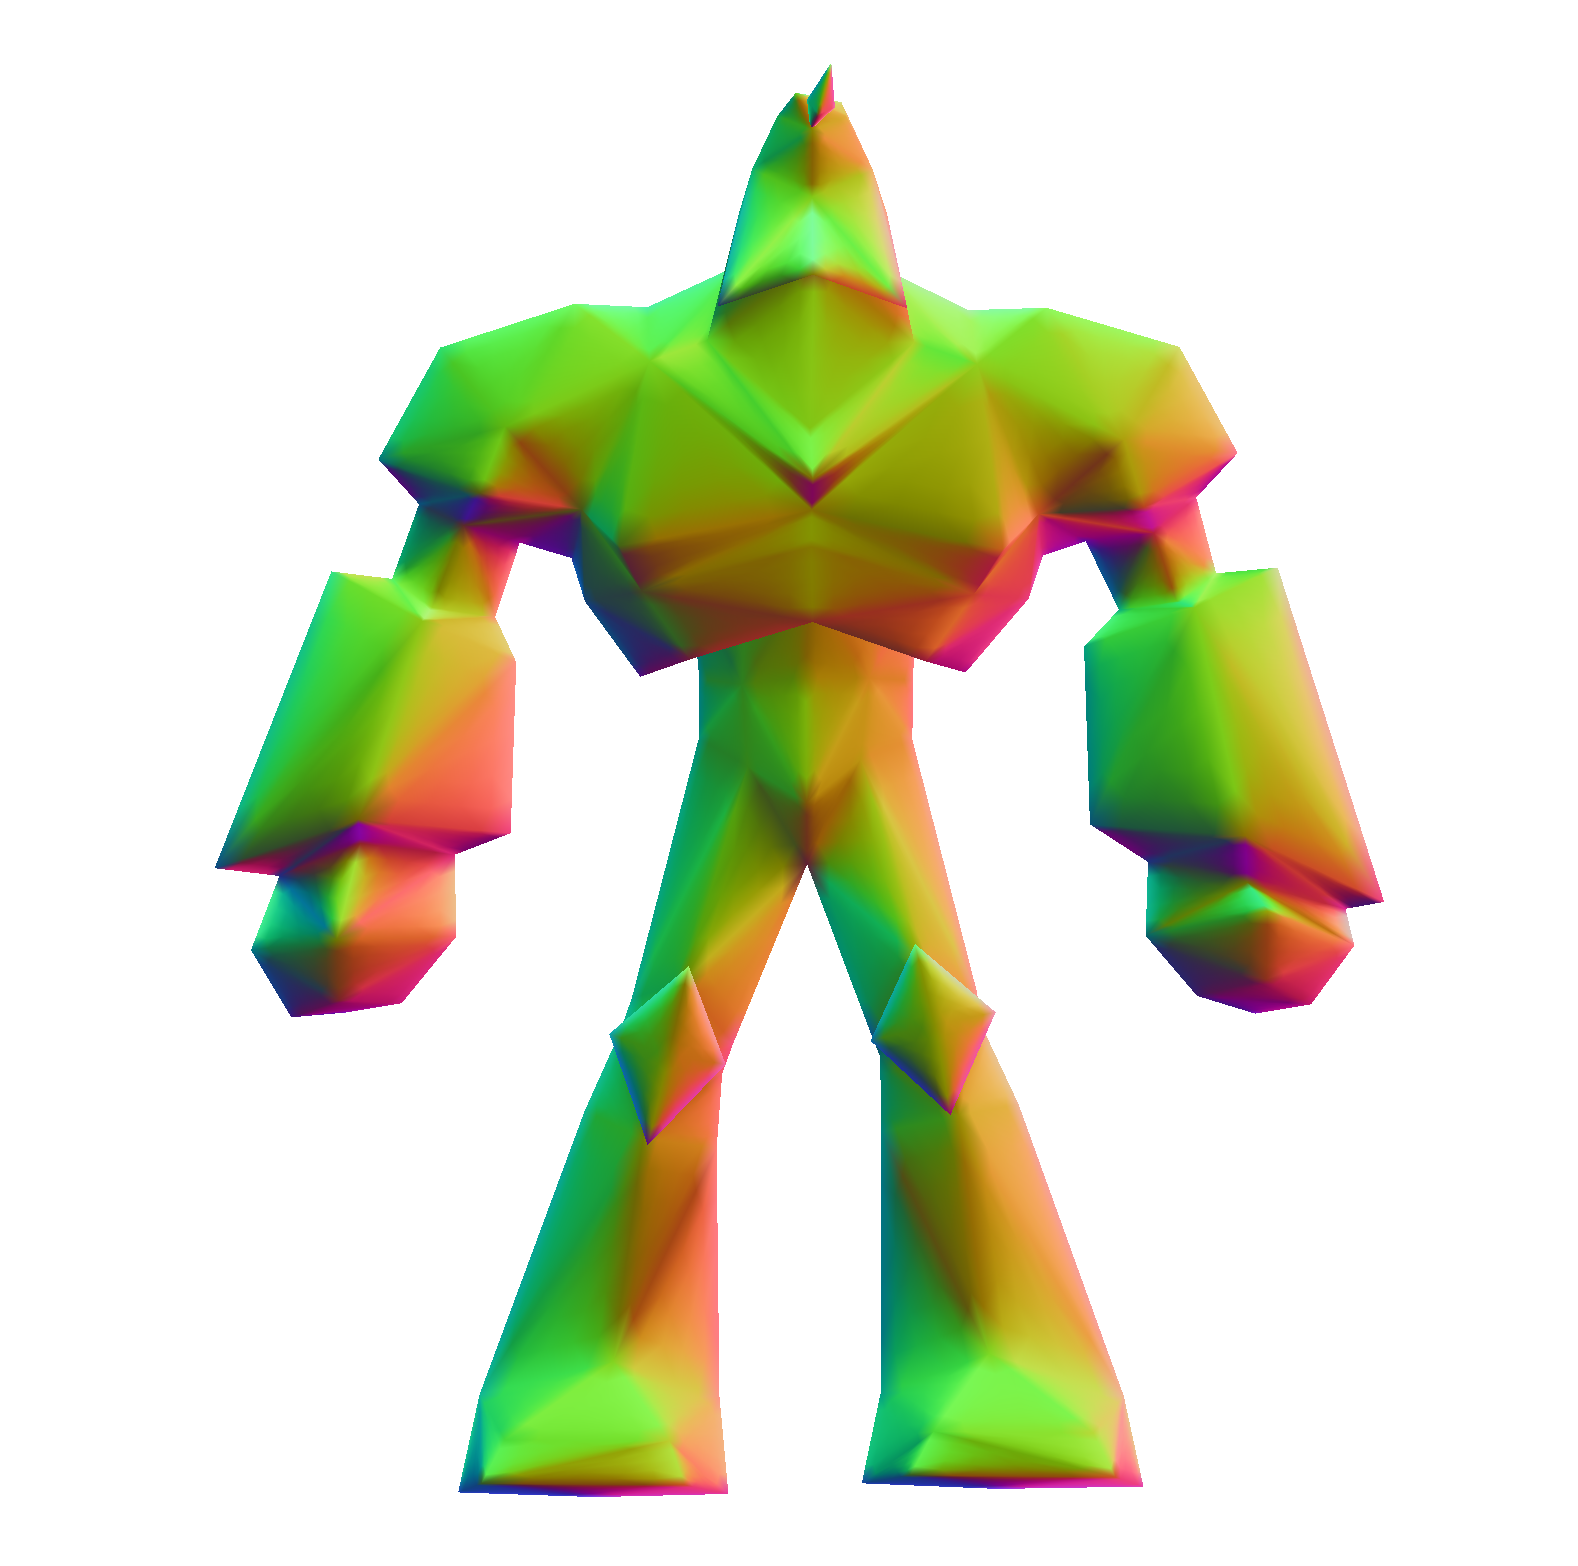
\includegraphics[width=\textwidth]{enforcer_normals_pn_i5_o5.png}
	\caption{The mesh rendered with point-normal triangles, colored based on the normals. Both the inner and outer tessellation level are set to 5. Note how much more defined the model seems when compared with \cref{fig:enforcerNormals}.}
	\label{fig:enforcerNormals5}		
\end{figure}

\begin{figure}
	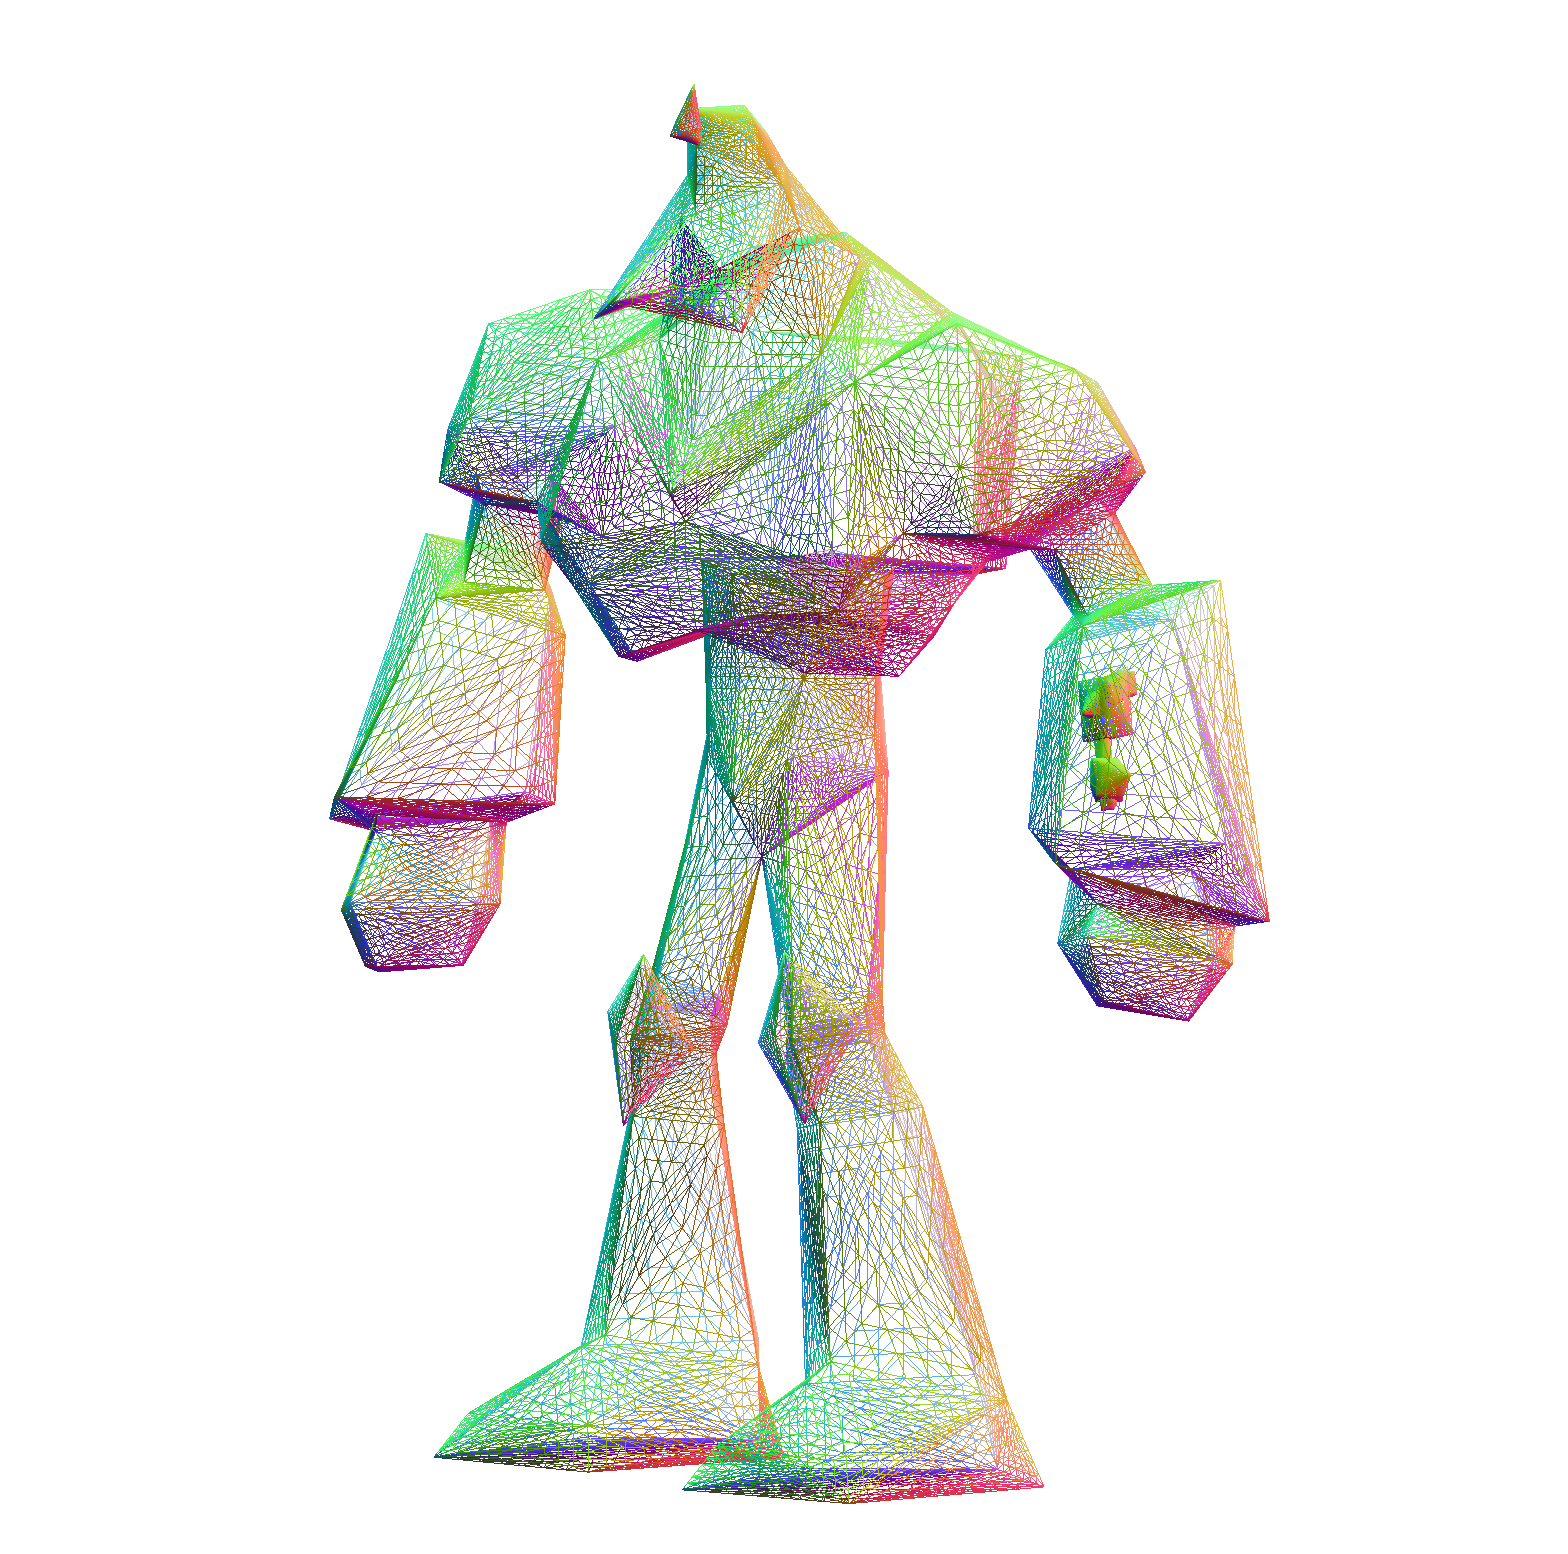
\includegraphics[width=\textwidth]{enforcer_normals_pn_i7_o7.png}
	\caption{The mesh rendered with point-normal triangles, colored based on the normals. Both the inner and outer tessellation level are set to 7. Note how much finer the wire frame is when compared with the one in \cref{fig:enforcerWireframe}.}		
	\label{fig:enforcerNormals7}	
\end{figure}

\begin{figure}
	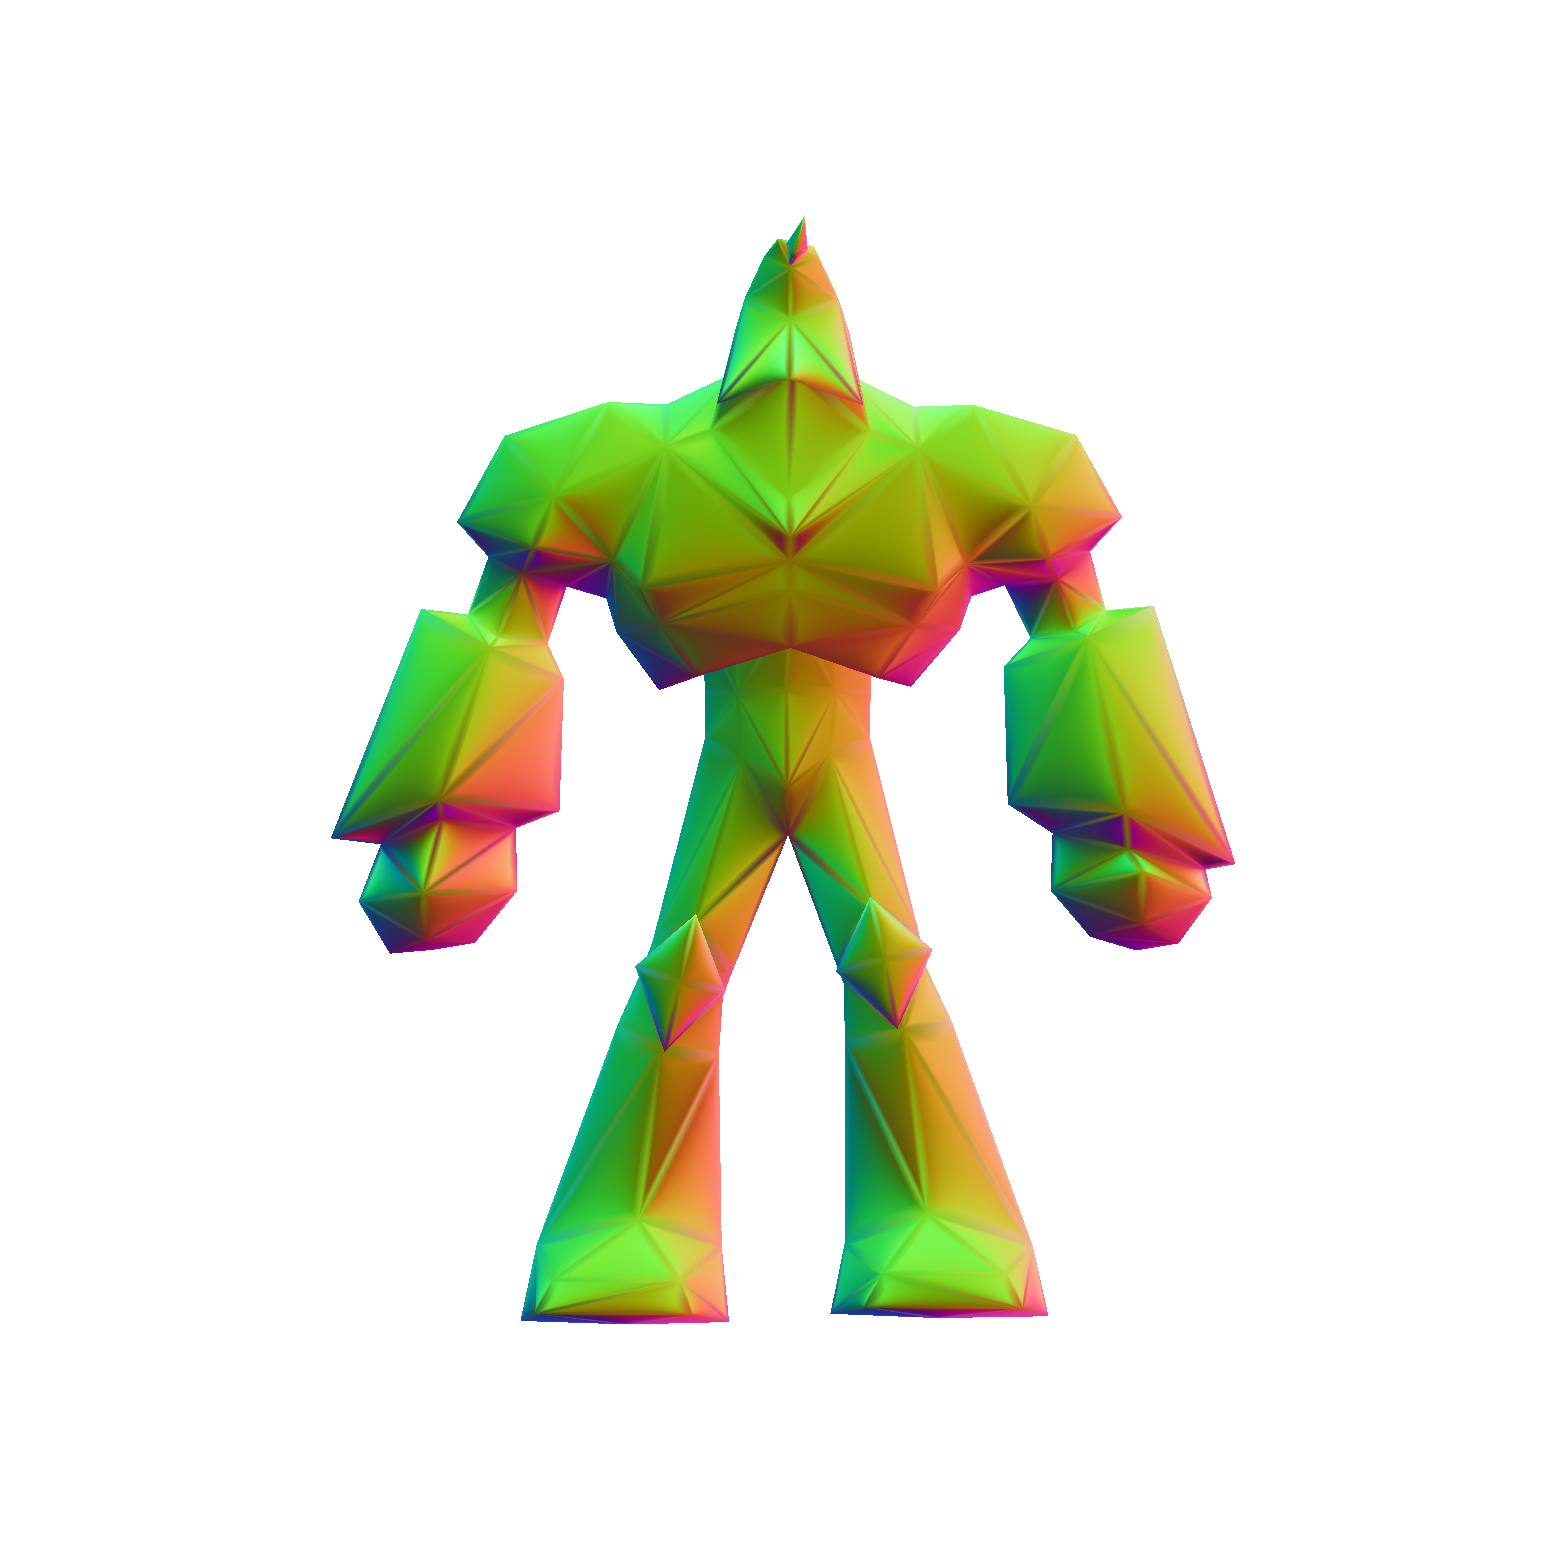
\includegraphics[width=\textwidth]{enforcer_normals_pn_i9_o1.png}
	\caption{The mesh rendered with point-normal triangles, colored based on the normals. Both the inner tessellation level set to 9 and the outer tessellation level set to 1. Note how the contours of the model do not differ from the ones in \cref{fig:enforcerFlat}, but how the the model is visually more pleasing than the one in \cref{fig:enforcerNormals}.}	
\end{figure}

\begin{figure}
	\centering
	\begin{subfigure}{\textwidth}
		\centering
		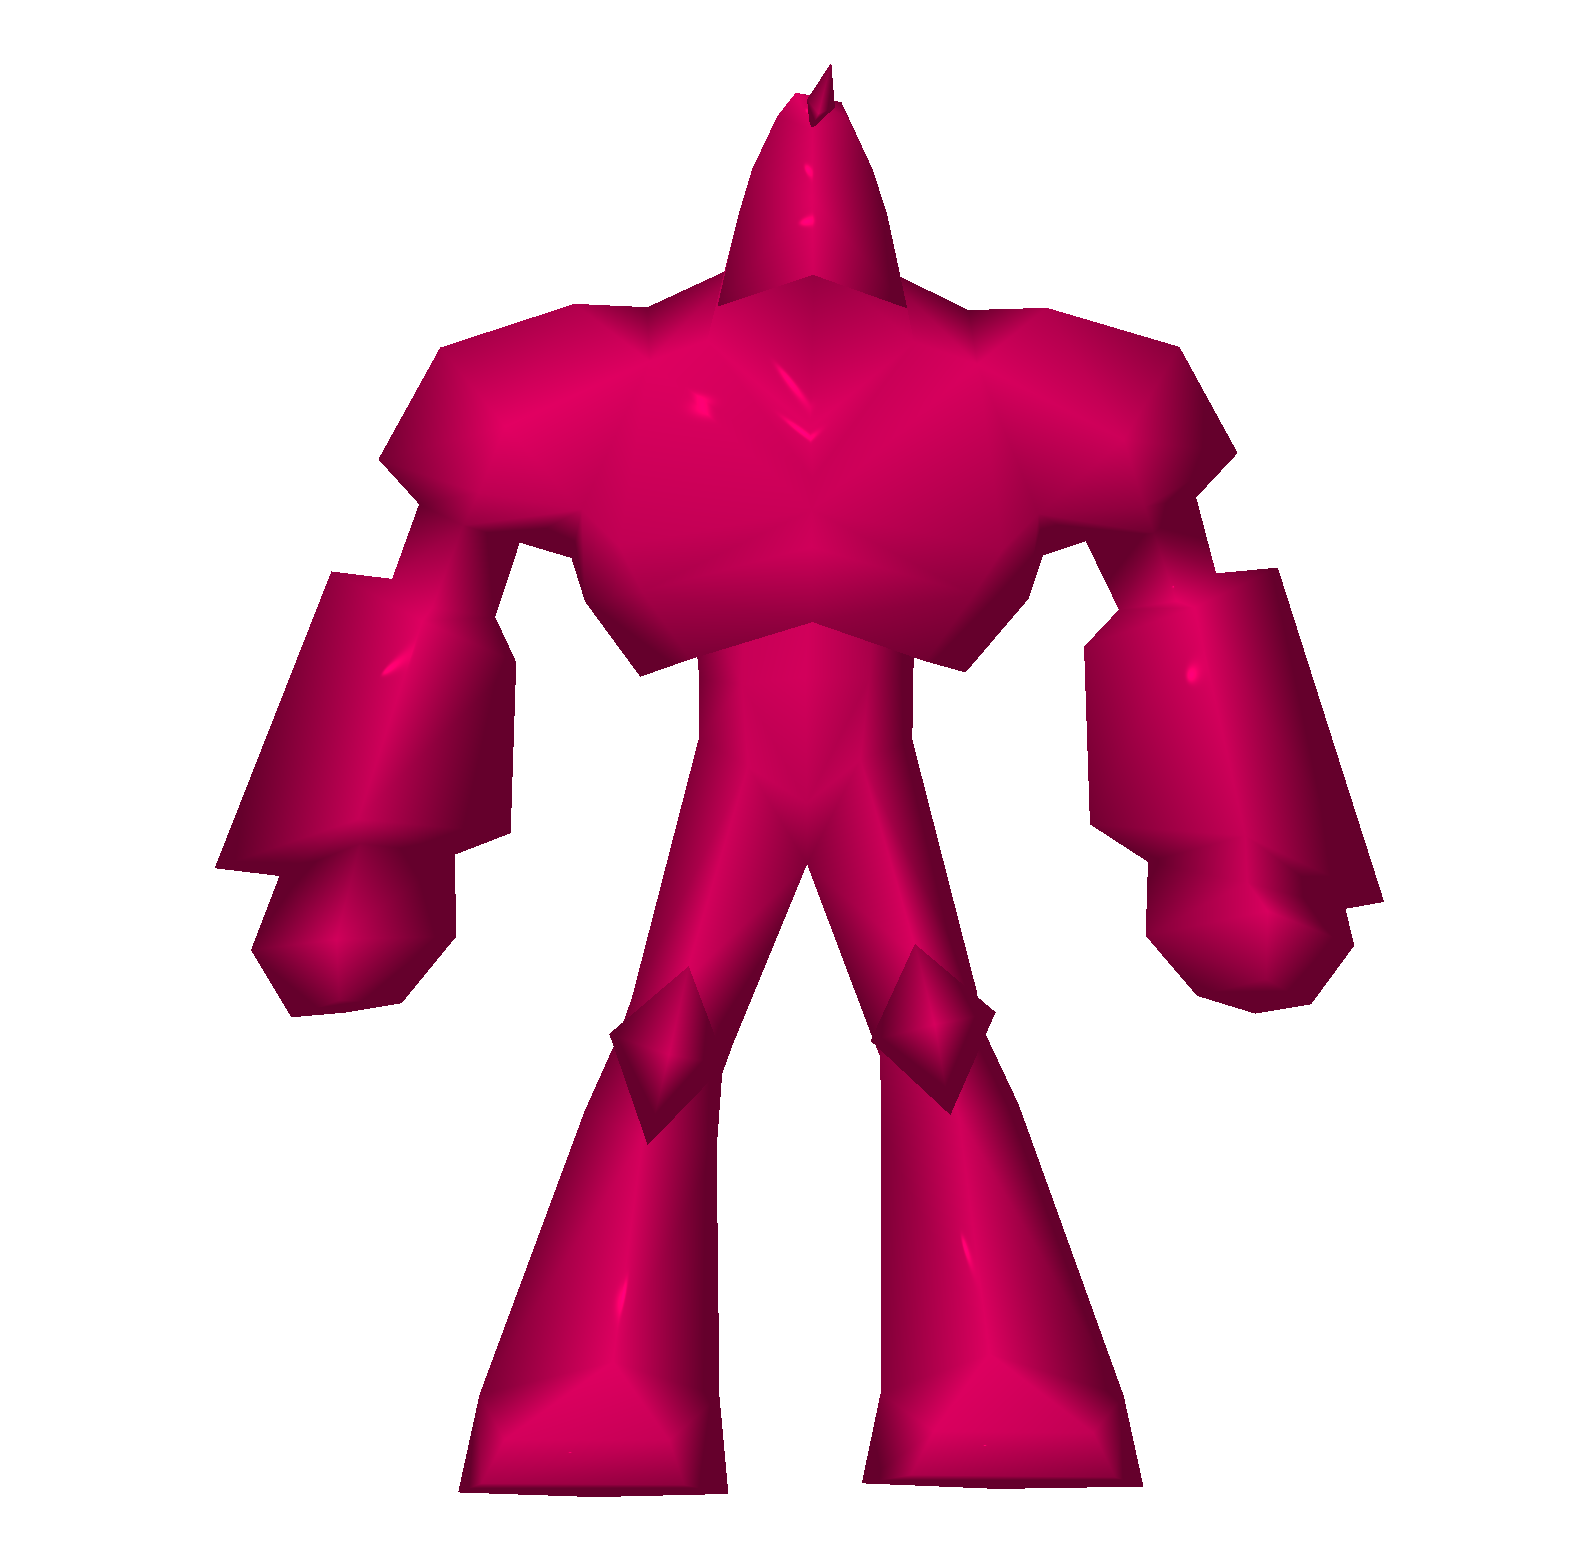
\includegraphics[width=\textwidth, height=0.26\textheight, keepaspectratio=true]{enforcer_phong_phong.png}
		\caption{Inner = 1, outer = 1}
		\label{fig:phong:i1o1}
	\end{subfigure}	
	\begin{subfigure}{\textwidth}
		\centering
		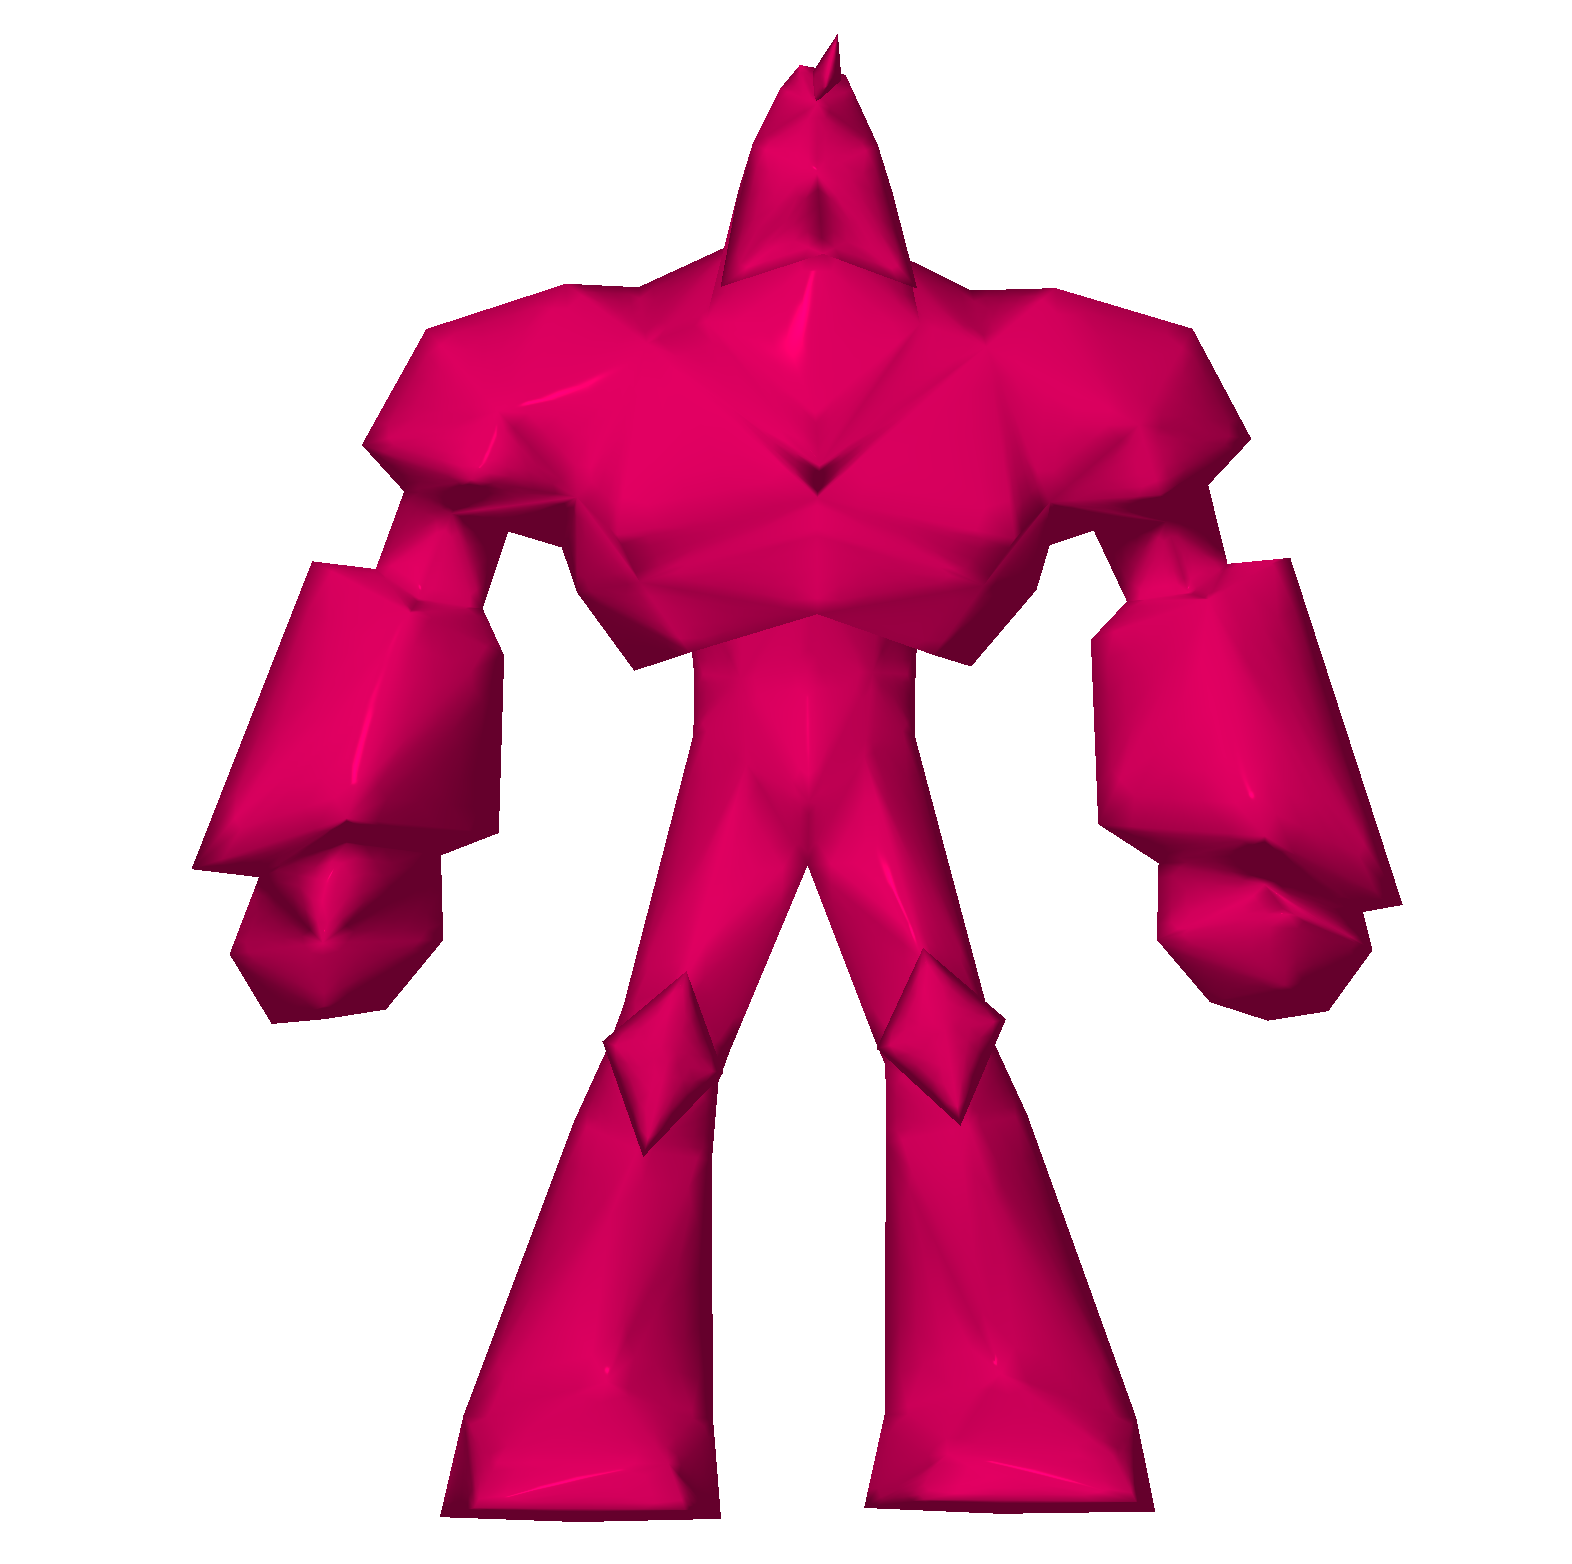
\includegraphics[width=\textwidth, height=0.26\textheight, keepaspectratio=true]{enforcer_phong_phong_pn_i5_o5.png}
		\caption{Inner = 5, outer = 5}
		\label{fig:phong:i5o5}
	\end{subfigure}
	\begin{subfigure}{\textwidth}
		\centering
		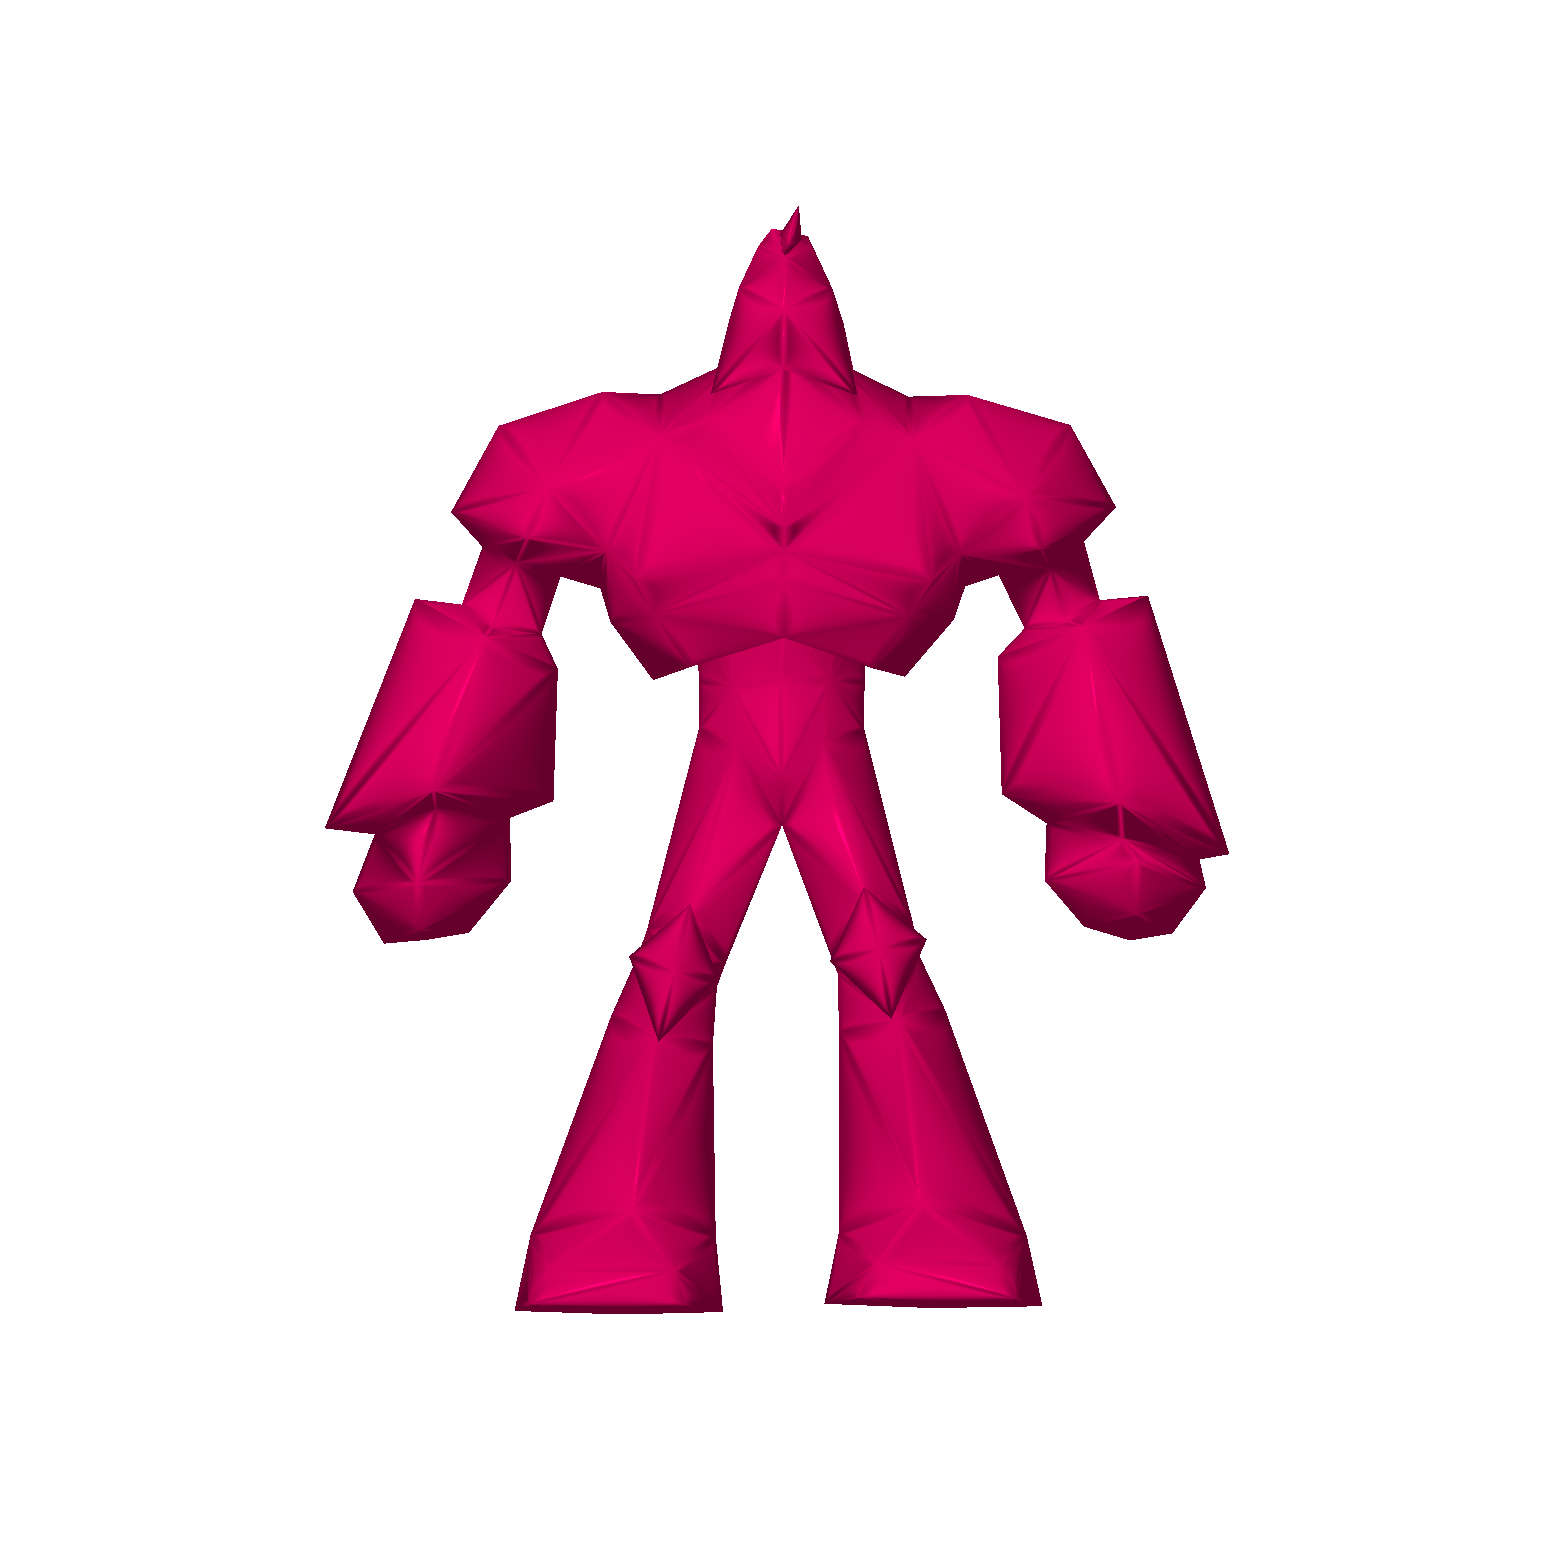
\includegraphics[width=\textwidth, height=0.26\textheight, keepaspectratio=true]{enforcer_phong_phong_pn_i9_o1.png}
		\caption{Inner = 9, outer = 1}
		\label{fig:phong:i9o1}
	\end{subfigure}	
	\caption{Phong shaded rendering of different point-normal meshes, based on the point-normal normals. Note how \subref{fig:phong:i5o5} the point-normal triangle model, is visually more pleasing than \subref{fig:phong:i1o1} the model that does not use point-normal triangles. \ref{fig:phong:i9o1} shows the strange effects that occur when the inner tessellation level is much higher than the outer tessellation level. This is especially visible in the shoulders of this model.}
	\label{fig:phong}
\end{figure}


\end{document}